\documentclass[fleqn]{article}
\usepackage[utf8]{inputenc}
\usepackage[margin=2.5cm]{geometry}

% bibliography
\usepackage[round, sort&compress]{natbib}
\usepackage{har2nat}
\bibliographystyle{agsm}

% custom header/footer
\usepackage{fancyhdr}
\pagestyle{fancy}
\renewcommand{\headrulewidth}{0pt}
\fancyhf{}
\rfoot{\textsf{\thepage}}
\lfoot{\textsf{Suzie Brown}}

% miscellaneous formatting
\usepackage{xcolor}
\usepackage[font=small]{caption}
\usepackage{subcaption}
\usepackage{enumitem}

% tikz
\usepackage{tikz}
\usetikzlibrary{positioning}

% pseudocode
\usepackage{algorithm}
\usepackage{algorithmicx}
\usepackage{algpseudocode}

% maths
\usepackage{amsmath}
\usepackage{amssymb}
\usepackage{amsthm}
\newtheorem{lemma}{Lemma}
\newtheorem{corollary}{Corollary}
\theoremstyle{definition}
\newtheorem{defn}{Definition}

% useful math symbols
\newcommand{\PR}{\mathbb{P}}
\newcommand{\E}{\mathbb{E}}
\newcommand{\V}{\operatorname{Var}}
\newcommand{\eqdist}{\overset{d}{=}}
\newcommand{\I}[1]{\mathbb{I}_{\{#1\}}}
\newcommand{\Ntoinfty}{\overset{N\to\infty}{\longrightarrow}}
\newcommand{\limNtoinfty}{\underset{N\to\infty}{\lim}}
\newcommand\indep{\protect\mathpalette{\protect\independenT}{\perp}}
\def\independenT#1#2{\mathrel{\rlap{$#1#2$}\mkern2mu{#1#2}}}

% distributions
\newcommand{\Cat}{\operatorname{Categorical}}
\newcommand{\Unif}{\operatorname{Uniform}}
\newcommand{\Mn}{\operatorname{Multinomial}}
\newcommand{\Bin}{\operatorname{Binomial}}

% project-specific commands
\newcommand{\F}{\mathcal{F}_{t-1}}
\newcommand{\vt}[2][t]{v_{#1}^{(#2)}}
\newcommand{\wt}[2][t]{w_{#1}^{(#2)}}
\newcommand{\wbar}[2][t]{\bar{w}_{#1}^{(#2)}}
\newcommand{\vttilde}[2][t]{\tilde{v}_{#1}^{(#2)}}

\title{Comparing expected coalescence rates for multinomial \& residual resampling}
\author{Suzie Brown}
\date{\today}

\begin{document}
\maketitle
\thispagestyle{fancy}

\section*{Case $N=2$}
\begin{lemma}
For all weight vectors $\wt{1:2}$, 
$\E[c_2^m(t) |\wt{1:2}] \geq \E[c_2^r(t) |\wt{1:2}]$.
\end{lemma}

\begin{proof}
With only $N=2$ particles, the coalescence rate becomes
\begin{equation*}
\E[c_N(t) |\wt{1:2}] = \frac{1}{(N)_2} \sum_{i=1}^{N} \E\left[ (\vt{i})_2 |\wt{1:2} \right] 
= \PR[\vt{1} = 0] + \PR[\vt{1} = 2].
\end{equation*}
For residual resampling,
\begin{equation*}
\E[c_2^r(t) |\wt{1:2}] = \I{\wt{1} \geq 1/2} (2\wt{1} -1) + \I{\wt{1} < 1/2} (2\wt{2} -1)
\end{equation*}
And for multinomial resampling,
\begin{align*}
\E[c_2^m(t) |\wt{1:2}] &= (\wt{1})^2 + (\wt{2})^2 \\
&= \I{\wt{1} \geq 1/2} ((\wt{1})^2 + (\wt{2})^2) + \I{\wt{1} < 1/2} ((\wt{1})^2 + (\wt{2})^2) \\
&\geq  \I{\wt{1} \geq 1/2} (\wt{1})^2 + \I{\wt{1} < 1/2} (\wt{2})^2
\end{align*}
Then since $(\wt{i} -1)^2 = (\wt{i})^2 -2\wt{i} +1 \geq 0$, we have that $(\wt{i})^2 \geq 2\wt{i} -1$ and hence we conclude the proof.
\end{proof}

\begin{center}
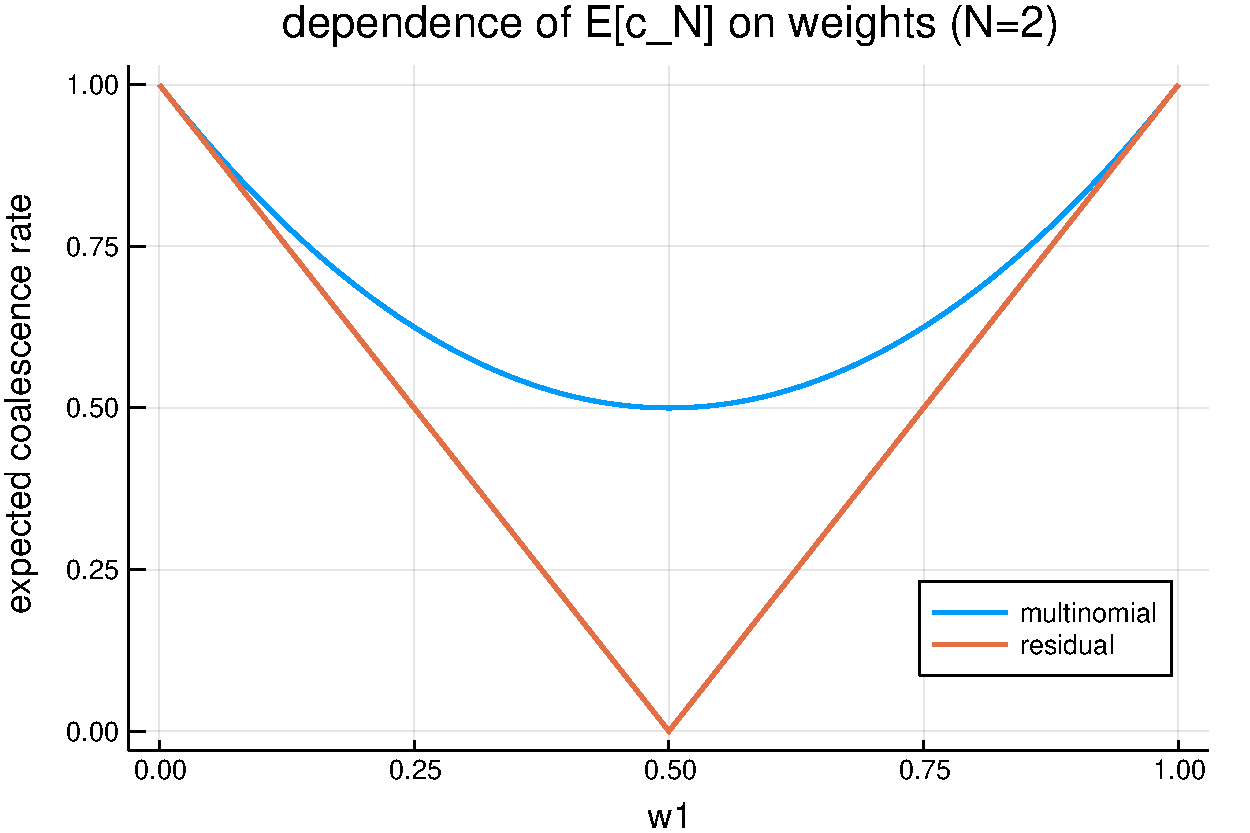
\includegraphics[width=0.8\textwidth]{plots/EcN_mn_res_N2.pdf}
\end{center}

%==================

\section*{Case $N=3$}
Given a weight vector $(\wt{1}, \wt{2}, \wt{3})$, let $w_{(1)} \geq w_{(2)} \geq w_{(3)}$ denote the weights sorted from high to low. 
With $N=3$ there are many more cases than with $N=2$, and these are described below, using the sorted weights.

In each case for the conditions on the sorted weights, the possible offspring count vectors (sorted in the same order as the weights) are listed, along with the probability of each (conditional on the given case). Finally, using these outcomes and associated probabilities, the conditional expectation of interest is calculated.\\

\begin{tabular}{ l | l | l | l | l }
Case & Weights & Offspring counts &  Conditional probabilities & $\E[c_2^r(t) | \wt{1:3}]$ \\
\hline
(A) & $w_{(1)} = 1$ & $(3,0,0)$ & 1 & 1 \\
\hline
(B) & $2/3 < w_{(1)} < 1$ & $(3,0,0)$ & $3w_{(1)} - 2$ & $2w_{(1)} -1$\\
	&& $(2,1,0)$ & $3w_{(2)}$ & \\
	&& $(2,0,1)$  & $3w_{(3)}$ & \\
\hline
(C) & $w_{(1)}=2/3$ & $(2,1,0)$ & $3w_{(2)}$ & 1/3 \\
	&& $(2,0,1)$ & $3w_{(3)}$ & \\
\hline
(D1) & $1/3 < w_{(1)} < 2/3$ and & $(2,1,0)$ & $3w_{(1)} - 1$ & $1/3 - w_{(3)}$ \\
	& $1/3 \leq w_{(2)} < 2/3$ & $(1,2,0)$ & $3w_{(2)} -1$ & \\
	&& $(1,1,1)$ & $3w_{(3)}$  & \\
\hline
(D2) &  $1/3 < w_{(1)} < 2/3$ and & $(3,0,0)$ & $(3/2)^2 (w_{(1)} - 1/3)^2$ & $ (1/4) (3w_{(1)} - 1)(w_{(1)} + 1)$ \\
	& $w_{(2)} < 1/3$ & $(2,1,0)$ & $(3/2)^2 2(w_{(1)} - 1/3)w_{(2)}$ &\\
	&& $(2,0,1)$ & $(3/2)^2 2(w_{(1)} - 1/3)w_{(3)}$ &\\
	&& $(1,2,0)$ & $(3/2)^2 w_{(2)}^2$ &\\
	&& $(1,0,2)$ & $(3/2)^2 w_{(3)}^2$ &\\
	&& $(1,1,1)$ & $(3/2)^2 2w_{(2)} w_{(3)}$ &\\
\hline
(E) & $w_{(1)} = 1/3$ & $(1,1,1)$ & 1 & 0 \\
\end{tabular}

\vspace{0.6cm}

\begin{lemma}
For all weight vectors $\wt{1:3}$, 
$\E[c_3^r(t) |\wt{1:3}] \leq \E[c_3^m(t) |\wt{1:3}]$.
\end{lemma}
\begin{proof}
We have the following expression in the case of residual resampling:
\begin{align*}
\E[c_3^r(t) |\wt{1:3}] &= (2w_{(1)} -1) \I{2/3 \leq w_{(1)} \leq 1} \\
&\qquad + (1/3 - w_{(3)}) \I{1/3 \leq w_{(1)} < 2/3} \I{1/3 \leq w_{(2)} < 2/3} \\
&\qquad + (1/4)(3w_{(1)} -1)(w_{(1)} +1) \I{1/3 \leq w_{(1)} < 2/3} \I{w_{(2)} <1/3}
\end{align*}
compared to the following in the case of multinomial resampling:
\begin{align*}
\E[c_3^m(t) |\wt{1:3}] &= w_{(1)}^2 + w_{(2)}^2 + w_{(3)}^2 \\
&= (w_{(1)}^2 + w_{(2)}^2 + w_{(3)}^2) \I{2/3 \leq w_{(1)} \leq 1} \\
&\qquad + (w_{(1)}^2 + w_{(2)}^2 + w_{(3)}^2) \I{1/3 \leq w_{(1)} < 2/3} \I{1/3 \leq w_{(2)} < 2/3} \\
&\qquad + (w_{(1)}^2 + w_{(2)}^2 + w_{(3)}^2) \I{1/3 \leq w_{(1)} < 2/3} \I{w_{(2)} <1/3}.
\end{align*}
Hence it suffices to show the following:
\begin{enumerate}[label=(\roman*)]
\item $(2w_{(1)} -1) \leq (w_{(1)}^2 + w_{(2)}^2 + w_{(3)}^2)$
\item $ (1/3 - w_{(3)}) \leq (w_{(1)}^2 + w_{(2)}^2 + w_{(3)}^2)$
\item $ (1/4)(3w_{(1)} -1)(w_{(1)} +1) \leq (w_{(1)}^2 + w_{(2)}^2 + w_{(3)}^2)$\\
\end{enumerate}
First consider (ii). Since $w_{(3)}$ is defined as the smallest of the three weights, we know that $w_{(3)} \in [0,1/3]$. Meanwhile, the RHS is the sum of the squared weights, which is always between 1/3 and 1. Therefore (ii) is true.\\[7pt]
Now let us consider (i). We have the identity $(w_{(1)} -1)^2 = w_{(1)}^2 -2w_{(1)} +1$, which implies that $w_{(1)}^2 \geq 2_w{(1)} - 1$. Since $w_{(2)}^2 + w_{(3)}^2 \geq 0$ we can therefore conclude that (i) is true.\\[7pt]
Finally consider (iii). In this case it is sufficient to show that $(1/4)(3w_{(1)} -1)(w_{(1)} +1) \leq w_{(1)}^2$. Note that
\begin{align*}
& w_{(1)}^2 - \frac{1}{4}(3w_{(1)} -1)(w_{(1)} +1) \\
& = \frac{1}{4} w_{(1)}^2- \frac{1}{2} w_{(1)} + \frac{1}{4} \\
& = \frac{1}{4} (w_{(1)} -1)^2 \geq 0.
\end{align*}
Therefore (iii) is also true, concluding the proof.
\end{proof}

\begin{figure}
	\centering
	\begin{subfigure}{\textwidth}
		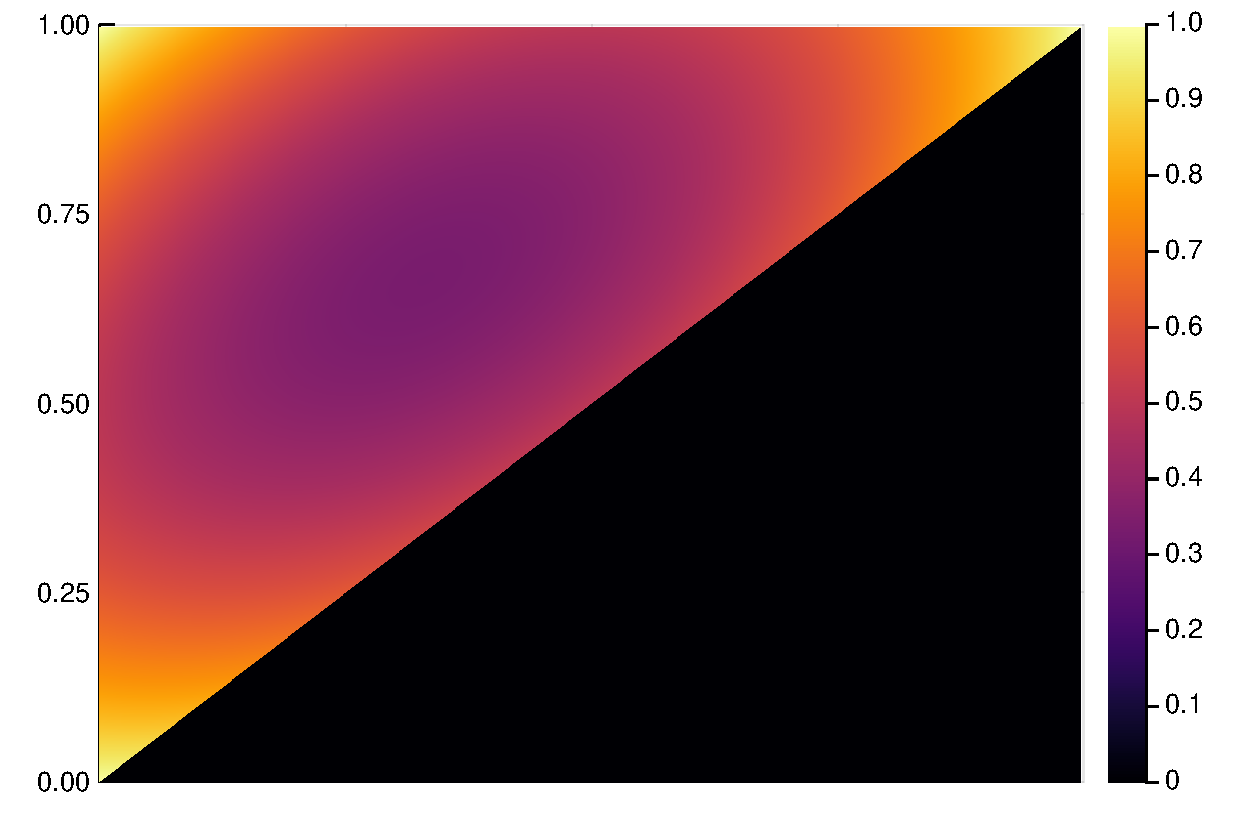
\includegraphics[width=0.5\textwidth]{plots/EcN_mn_N3_heatmap.pdf}
		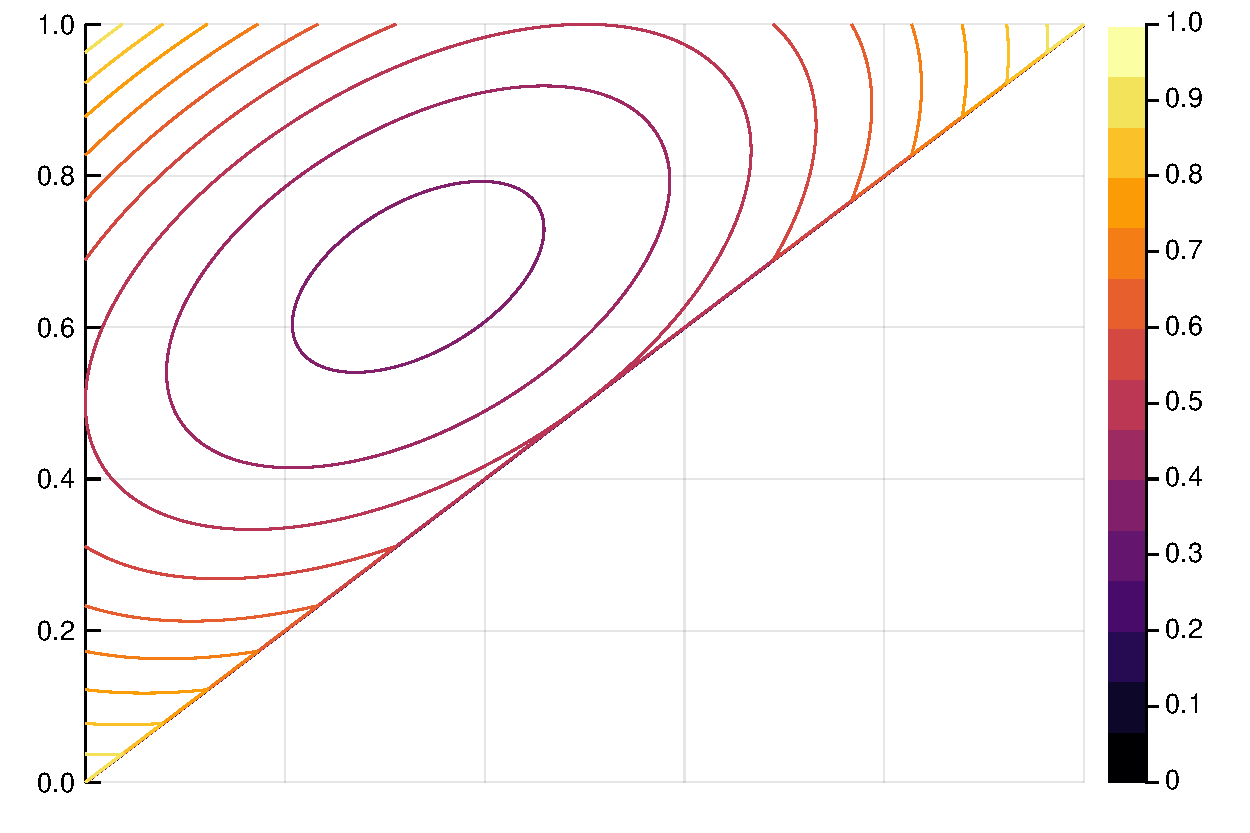
\includegraphics[width=0.5\textwidth]{plots/EcN_mn_N3_contour.pdf}
	\caption{Expected coalescence rate with multinomial resampling ($N=3$)}
	\end{subfigure}
	\begin{subfigure}{\textwidth}
		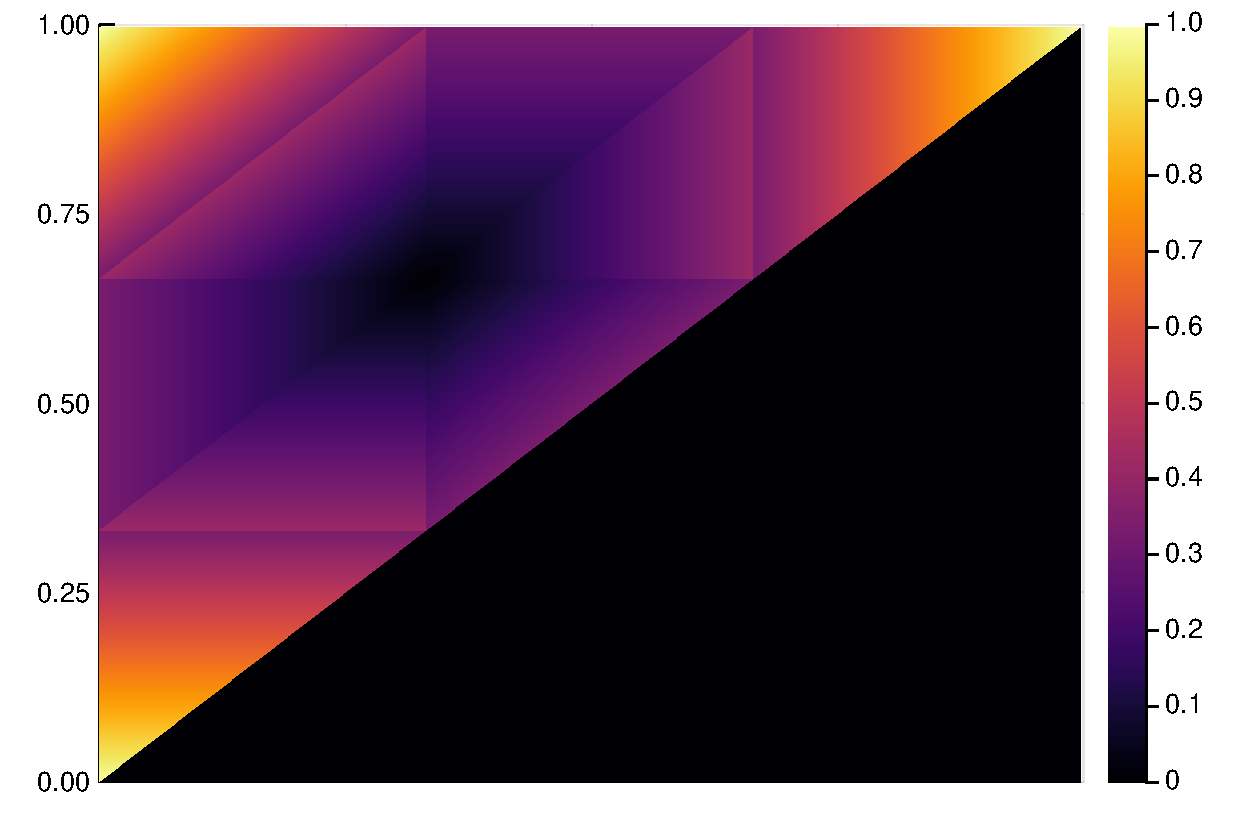
\includegraphics[width=0.5\textwidth]{plots/EcN_res_N3_heatmap.pdf}
		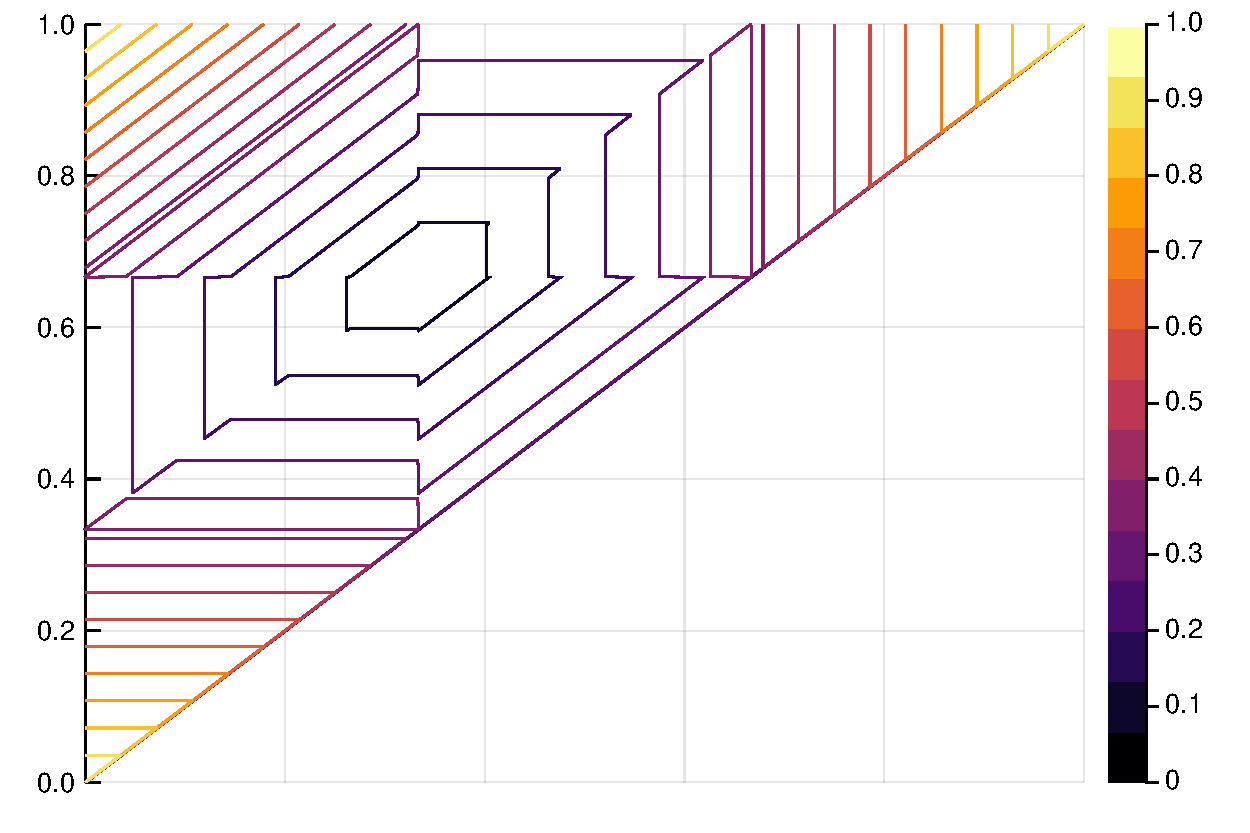
\includegraphics[width=0.5\textwidth]{plots/EcN_res_N3_contour.pdf}
	\caption{Expected coalescence rate with residual resampling ($N=3$)}
	\end{subfigure}
	\begin{subfigure}{\textwidth}
		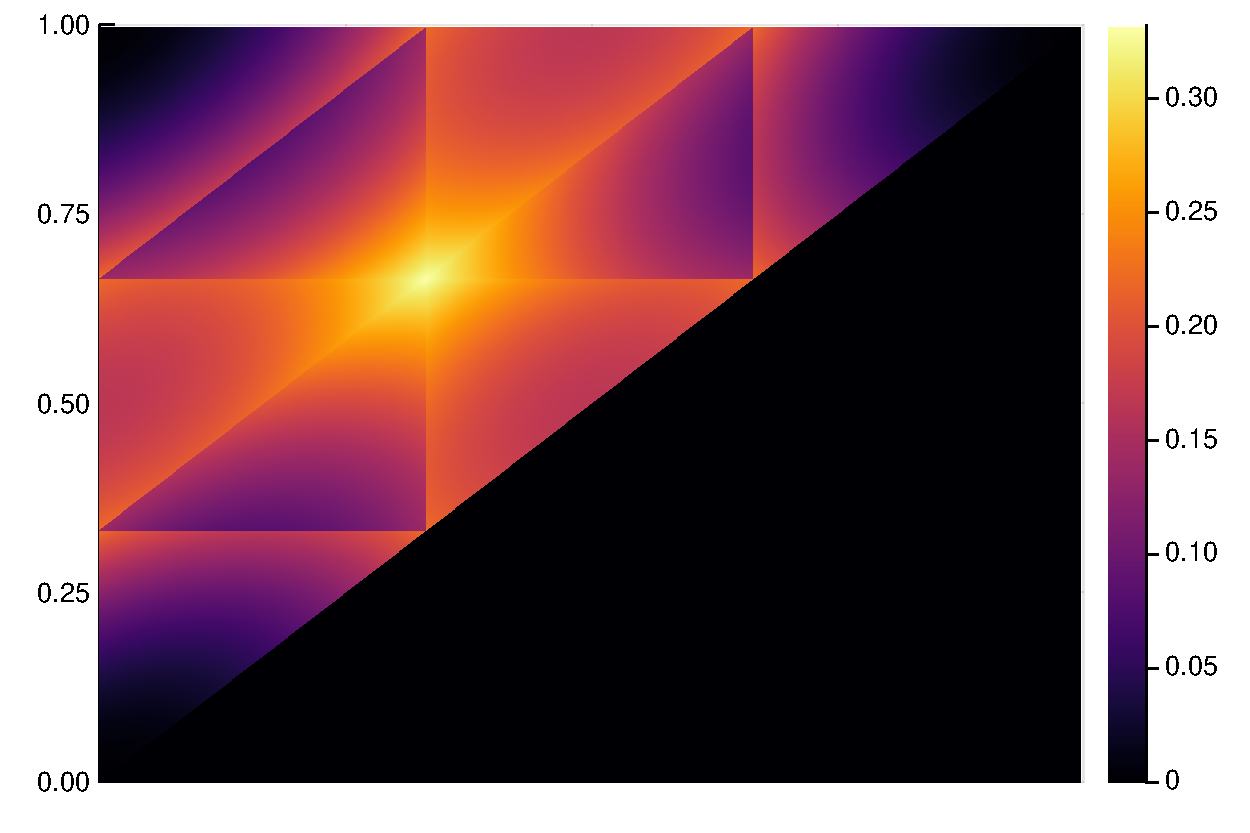
\includegraphics[width=0.5\textwidth]{plots/EcN_mn_res_diff_N3_heatmap.pdf}
		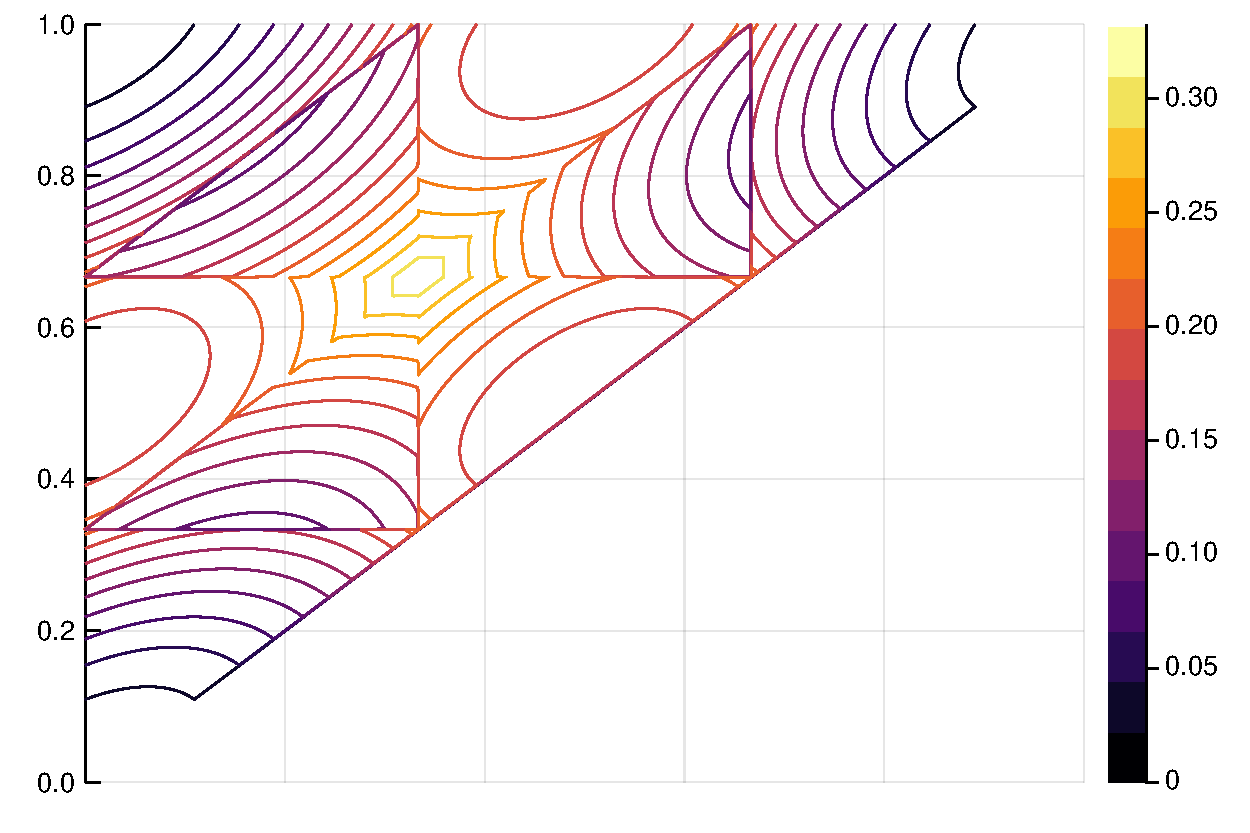
\includegraphics[width=0.5\textwidth]{plots/EcN_mn_res_diff_N3_contour.pdf}
	\caption{Difference between expected coalescence rate with multinomial or residual resampling ($N=3$)}
	\end{subfigure}
\end{figure}


\end{document}